\chapter{Cycles in the Collatz Graph}
\label{ch:cycles}

\section{A remark about cycles}
\label{sec:cycles}
In graph theory, a path of length $n\geq 1$ that starts and ends at the same vertex is called a circuit. A circuit, in which no vertex is repeated with the sole exception that the initial vertex is the terminal vertex, is called a cycle. A cycle of length $n$ is referred to as an $n$-cycle. For these definitions, we rely on \cite[p.~599]{Ref_Rosen}, \cite[p.~35]{Ref_Benjamin_Chartrand_Zhang} and \cite[p.~445]{Ref_Chartrand_Zhang}. Furthermore, we call a cycle originating from the root a trivial cycle.

\begin{remark}
In order for the cycles to become graphically visible, we now require that in a graph $H$ two vertices $v_1$ and $v_2$ are one and the same if the label of both nodes are identical: $l_{V(H)}(v_1)=l_{V(H)}(v_2)\rightarrow v_1=v_2$. As a consequence, there is no guarantee that the graph precisely refers to the algebraic structure of a free monoid anymore. A free monoid requires that each of its elements can be written in one and only one way.
\end{remark}

When different nodes collapse on one, the graph is no longer necessarily a tree. Let us point to the monoid $S^\ast$, which we introduced in section \ref{sec:groups_graphs}. Take for example four of its elements, the empty string $e$, the strings $qqr$, $qqrqqr$, and $qqrqqrqqr$. These elements lie as well within the subset $U\subset T\subset S^\ast$, and they are represented by nodes of the tree $H_U$ that all have the same label $1=ev_{S^\ast}(qqr,1)=ev_{S^\ast}(qqrqqr,1)=ev_{S^\ast}(qqrqqrqqr,1)$. These nodes are one and the same, the root of $H_U$. Visually, then in $H_U$ a directed edge goes from the vertex labeled with $4$ back to the root node. Analogically, in $H_{C,3}$ a loop connects the root to itself, since due to the path contraction even labeled nodes do not exist in $H_{C,3}$. The  aforementioned example reflects the trivial cycle of the Collatz sequence.

Figure~\ref{fig:5} depicts a section of $H_{C,5}$, which includes the $3$-cycle $43,17,27$. Because of the two non-trivial cycles $(43,17,27)$ and $(83,33,13)$, in $H_{C,5}$ there does not exist a path between the root and the vertex $43$ and between the root and the vertex $83$. Hence, $H_{C,5}$ is said to be a disconnected graph. Generally, a graph is called a disconnected graph if it is impossible to walk (along its edges) from any vertex to any other \cite[pp.~46-47]{Ref_Benjamin_Chartrand_Zhang}.

\begin{figure}
	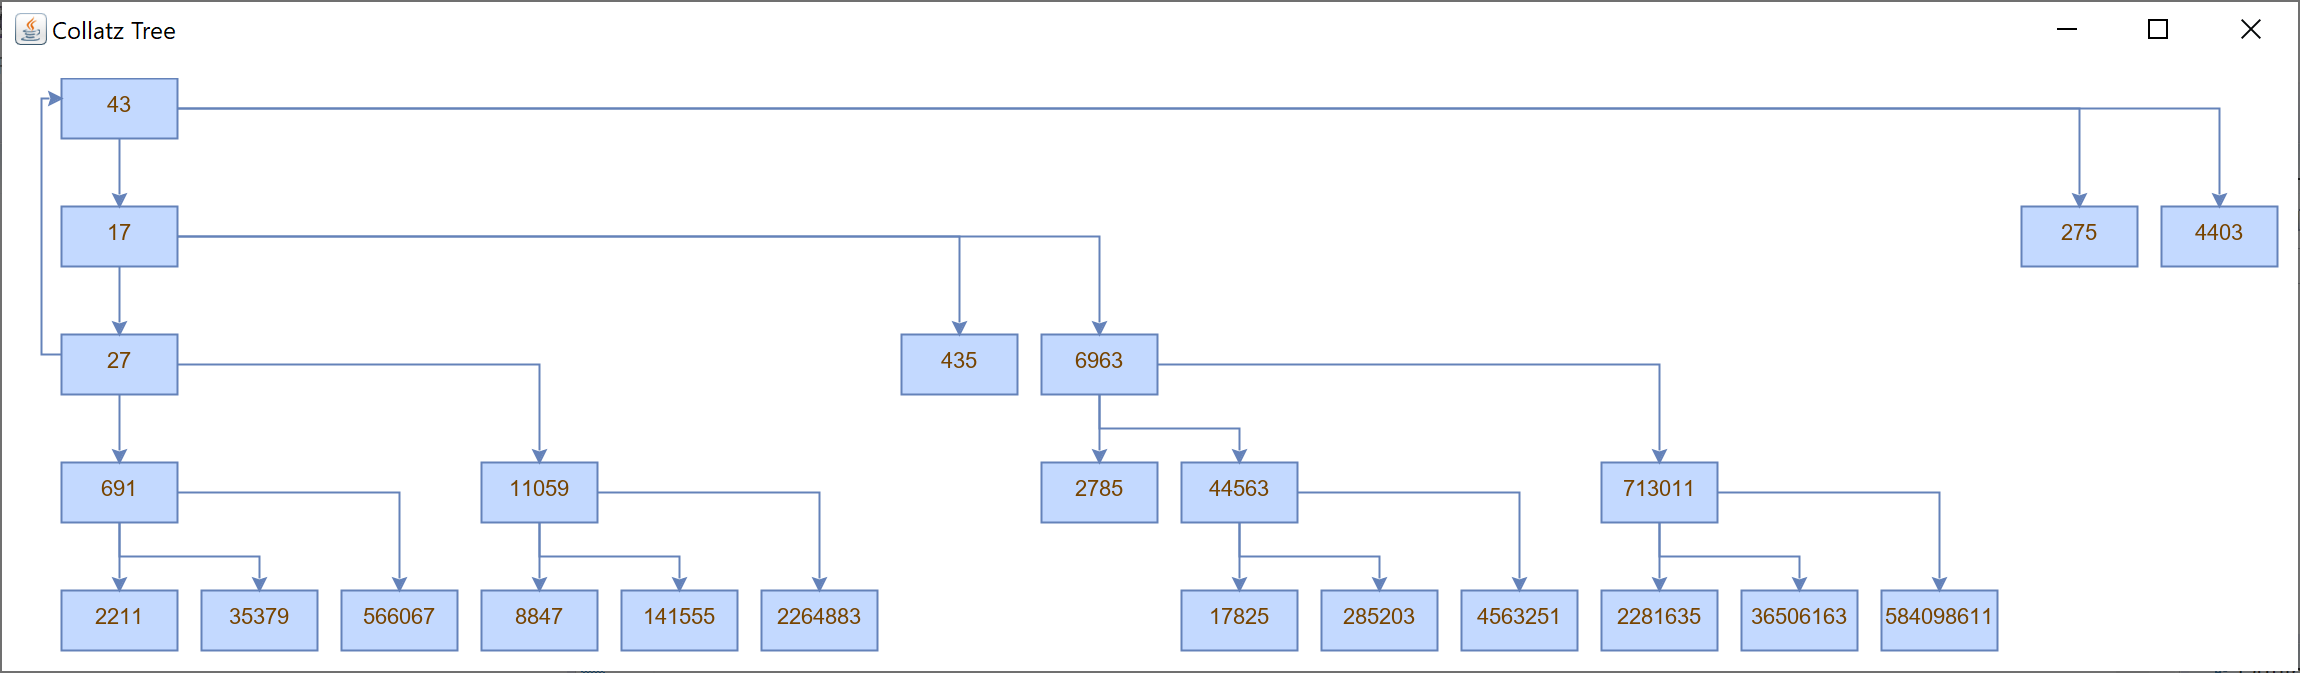
\includegraphics[width=1.00\textwidth]{figures/h_c5a.png}
	\caption{Section of $H_{C,5}$ including the $3$-cycle $43,17,27$}
	\label{fig:5}
\end{figure}

The following considerations focus on non-trivial cycles, and therefore on cycles that do not originate from the root, but cause the graph to be a disconnected graph. Utilizing the example of the graph $H_{C,5}$ we are able to deduct from the cycle $(43,17,27)$ the simple and self-evident equality $\textit{left-child}^3(43)=43$:
\begin{equation*}
\begin{array}{l}
\textit{left-child}(43)=\frac{1}{5}*\left(43*2^1-1\right)=17
\\[\medskipamount]
\textit{left-child}(17)=\frac{1}{5}*\left(17*2^3-1\right)=27
\\[\medskipamount]
\textit{left-child}(27)=\frac{1}{5}*\left(27*2^3-1\right)=43
\end{array}
\end{equation*}

Obviously, the authors note, it would be interesting to find out what circumstances enable a graph to have non-trivial cycles, whether it be the $5x+1$ variant, the $7x+1$ variant of $H_C$ or any variant $H_{C,k}$ with $k\geq 1$.

\section{\texorpdfstring{Which variants of $H_C$ have non-trivial cycles?}{Which variants of HC have non-trivial cycles?}}
\label{sec:non_trivial_cycles}
The generalization of the relationship between successive nodes, given by equation~\ref{eq:generalized_reachability} leads to the condition for an existence of an $n$-cycle in any $kx+1$ variant of $H_C$, which looks analogous to the condition given by equation~\ref{eq:func_cycle} that specifies $H_{C,3}$ has a cycle:
\begin{equation}
\label{eq:generalized_cycle}
2^\alpha=\prod_{i=1}^{n}\left(k+\frac{1}{v_i}\right)
\end{equation}

The natural number $\alpha$ is the sum of edges that have been contracted between the vertices $v_i$ forming the cycle, in other words $\alpha$ is the number of divisions by $2$ within the sequence. The natural number $n$ is the cycle length and $k$ obviously specifies the variant of $H_C$. Since between each vertex at least one edge has been contracted (at least one division by $2$ took place), we know that our exponent alpha is greater than or equal to the sequence length:
\begin{equation}
\label{eq:n_alpha}
\alpha\ge n
\end{equation}

In their 2020 publication Koch et al. \cite{Ref_Koch_2020} provide a list of cycles for different values of $k$, identified with a linear search performed by a Python script \cite{Ref_Koch_Github}. Table~\ref{table:known_cycles} lists all these discovered cycles (refer to \cite{Ref_Koch_2020} for details on the discovery procedure and search intervals). Note that the cycles in table~\ref{table:known_cycles} are written in reverse order, i.e. in the order which corresponds to the Collatz sequence. To obtain the cycles in terms of graph theory referring to the graph $H_C$, read them from right to left.

\begin{table}[H]
	\centering
	\begin{tabular}{|L|R|R|C|}
		\hline
		\thead{\boldsymbol{k}} &
		\thead{\textbf{cycle}} &
		\thead{\boldsymbol{\alpha}} &
		\thead{\textbf{non-trivial}} \\
		\hline
		1 &
		1 &
		1 &
		\\
		\hline
		3 &
		1 &
		2 &
		\\
		\hline
		5 &
		1,3 &
		5 &
		\\
		\hline
		5 &
		13,33,83 &
		7 &
		\checkmark \\
		\hline
		5 &
		27,17,43 &
		7 &
		\checkmark \\
		\hline
		7 &
		1 &
		3 &
		\\
		\hline
		15 &
		1 &
		4 &
		\\
		\hline
		31 &
		1 &
		5 &
		\\
		\hline
		63 &
		1 &
		6 &
		\\
		\hline
		127 &
		1 &
		7 &
		\\
		\hline
		181 &
		27,611 &
		15 &
		\checkmark \\
		\hline
		181 &
		35,99 &
		15 &
		\checkmark \\
		\hline
		255 &
		1 &
		8 &
		\\
		\hline
		511 &
		1 &
		9 &
		\\
		\hline
	\end{tabular}
	\caption{Known $n$-cycles in $kx+1$ variants of $H_C$ for $k\leq1000$, $n\leq 100$}
	\label{table:known_cycles}
\end{table}

Based on the results shown in table~\ref{table:known_cycles} we state the following theorem~\ref{theo:2} that renders more precisely the prerequisite for cycles that may occur in any variants of $H_C$.

\begin{theorem}
	\label{theo:2}
	An $n$-cycle can only exist in a graph $H_{C,k}$, if the following equation holds:
	\begin{equation*}
	2^{\bar\alpha}=2^{\lfloor n\log_2k\rfloor+1}=\prod_{i=1}^{n}\left(k+\frac{1}{v_i}\right)
	\end{equation*}
\end{theorem}

The statement behind theorem~\ref{theo:2} consists in the claim that, in order for an $n$-cycle to occur, the exponent $\alpha$ has to be $\bar\alpha=\lfloor n\log_2k\rfloor+1$. This statement is true if the following general condition for the validity of the cycle-alpha's upper limit always holds (see \cite{Ref_Koch_2020}):
\begin{equation}
\label{eq:condition_max}
n\log_2k-\lfloor n\log_2k\rfloor<2-\log_2\left(\prod_{i=1}^{n}\left(1+\frac{1}{kv_{i}}\right)\right)
\end{equation}

A product $\prod(1+a_n)$ with positive terms $a_n$ is convergent if the series $\sum a_n$ converges, see Knopp \cite[p.~220]{Ref_Knopp}. A similar statement provides Murphy \cite{Ref_Murphy}, who write the factors in the form $c_n=1+a_n$ and explains that if $\prod c_n$ is convergent then $c_n\rightarrow1$ and therefore if $\prod (1+a_n)$ is convergent then $a_n\rightarrow0$. Thus, to verify whether the product in condition~\ref{eq:condition_max} is converging towards a limiting value, it is sufficient to examine the following sum:
\begin{equation*}
\sum_{i=1}^{n}\frac{1}{kv_{i}}
\end{equation*}

The sum of reciprocal vertices depending only from $v_1$ is given in appendix~\ref{appx:sum_reciprocal_vertices}.
